\chapter{Operaciones cuánticas} % {{{
% Intro {{{
% \janote{\h{Hey Carlos.} Dejé los comentarios del esqueleto
% del capítulo para que recordaras lo que habíamos acordado.
% Intenté dar suficiente detalle para este capítulo para introducir
% las operaciones cuánticas, pero toma en cuenta que muchas cosas
% (demostraciones, detalles más formales) los deje por fuera pensando 
% que se pueden guardar para la tesis. Mi objetivo fue conectar 
% todo el capítulo motivado en ejemplos, que a mi parecer cumple
% con el objetivo de este trabajo.
% \newline}
% \janote{
% - Introducción hablando de que las operaciones cuánticas sirven 
% para describir la dinámica de los sistemas abiertos y una guía al 
% lector de qué se viene en este cap. Enfatizar en que el truco es 
% considerar como 'nuevo sistema cerrado' al sistema extendido}
% \cpnote{No entiendo esa frase}
% \janote{Me refiero a que un sistema que interactúa con su entorno es abierto, 
% pero si consideramos al sistema total (principal+entorno) ese es cerrado.
% \textbf{Ahora que lo expliqué ya no encuentro sentido para hablar de esto aquí,
% mejor lo voy a quitar}}

Las operación cuánticas son un marco teórico que proporcionan
una manera de describir el cambio dinámico de los estados 
de los sistemas cuánticos abiertos \cite{bengtsson_zyczkowski_2017}. 
En la naturaleza es imposible
encontrar un sistema cuántico perfectamente cerrado, es decir, un 
sistema cuántico ideal que no sufra de interacción con su entorno
\cite{nielsen_chuang_2011}. Los sistemas cuánticos reales 
interaccionan con su entorno y, peor aún, en el laboratorio 
los grados de libertad del entorno son, en general, inaccesibles.
Las operaciones cuánticas son un formalismo que consideran
la naturaleza abierta de los sistemas cuánticos reales y proporciona
las herramientas para describir de manera discreta la dinámica
de este tipo de sistemas.

En la sección 2.1 vamos a discutir la condición de completa 
positividad \cpnote{mejor diría algo de lo qe se pueda agarrar el lector. Algo asi 
como ``obtendremos las condiciones matemáticas necesarias para definir un 
canal válido'' o algo asi, porque si no el que no sepa, va a quedar confundido} de las operaciones cuánticas, motivando la definición
a partir de un ejemplo de una operación que deforma la esfera de
Bloch de 1 qubit a un disco. Las secciones 2.2 y 2.3 introducen dos 
representaciones distintas de las operaciones cuánticas,
vamos a mostrar la conexión entre ambas representaciones
mediante la matriz de Choi de una operación cuántica. Para 
concluir, en la sección 2.4 se ilustran tres ejemplos de 
operaciones cuánticas de 1 qubit que proporcionarán familiaridad
e intuición sobre los canales cuánticos. 
% }}}
\section{Mapeos completamente positivos} % {{{
% \janote{
% Introducir la transformación de la matriz de densidad $\rho$ y hablar
% de que $\E$ transforma estados en estados.\newline}
% \janote{
%     - Motivación de la CP. Ejemplo del mapeo que deforma la esfera de Bloch
%     en un disco: presentar que el mapeo extendido para 2 qubits
%     aplicado al estado máximamente entrelazado resulta en una matriz 
%     no positiva (algo que no es estado).\newline}
% \janote{- Definición de CP del Geometry of Quantum States.\newline}
% \janote{- Concluir con que las operaciones que estudiamos deben ser CPTP.
% \newline}
En el formalismo de las operaciones cuánticas un estado cuántico,
descrito por su operador de densidad $\rho$,
se transforma según la ecuación \cite{nielsen_chuang_2011}
\begin{align}
\rho' = \E (\rho)
\label{eq:E(rho)},
\end{align} 
donde $\E$ es una operación cuántica que representa alguna evolución 
física y $\rho'$ es el estado que resulta de la evolución\cpnote{Normalmente 
uno cita al final de la frase, a menos que no se entienda. En este caso y casi
siempre, funciona ponerla al final}.
En el capítulo anterior hemos 
establecido dos ejemplos de operaciones cuánticas: la evolución unitaria 
y la medición del estado de un sistema, 
para los cuales $\E \qty(\rho)=U\rho U^{\dagger}$ y 
$\E(\rho)=M\rho M^{\dagger}$\cpnote{Aca tienes un posible problema, porque 
entonecs no conservas la traza. Quizá yo quitaria ese ejemplo, o
pondría una suma mejor hablemos}, respectivamente. 
Una operación cuántica describe discretamente 
el cambio dinámico que un estado cuántico 
atraviesa durante un proceso físico. 

Una operación cuántica $\E$ es
una transformación lineal que mapea matrices de densidad en matrices 
de densidad \cite{bengtsson_zyczkowski_2017}. Surge entonces la siguiente
pregunta: si $\E$ es un mapeo afín de matrices de densidad, ¿eso es
suficiente para que $\E$ represente una operación física? 
La respuesta es que no, y el resto de esta sección está dedicada
explicar porqué y motivar la definición de completa positividad.  
Para que $\E$ sea una evolución física la operación debe de cumplir con dos
condiciones, ser un mapeo afín de matrices de densidad 
y satisfacer la condición de completa positividad. 

La necesidad de satisfacer la completa positividad
es consecuencia de la interacción que un sistema podría tener
con su entorno, sistema secundario que vamos 
a considerar inaccesible durante el resto del capítulo.
A continuación vamos a presentar un ejemplo que justificará la condición
de completa positividad de las operaciones cuánticas y, seguidamente,
vamos a finalizar con la definición precisa de esta condición.

Vamos a considerar una operación sobre el estado de un sistema de 
1 qubit. Luego, al considerar la extensión de la misma operación,
sobre el estado máximamente entrelazado de un sistema de 2 qubits, 
veremos que el estado resultante no es un estado físico
De esa manera, se justificará la condición de completa positividad 
de una operación cuántica para representar un proceso físico.

La matriz de densidad de 1 qubit se puede escribir convenientemente
como \cite{nielsen_chuang_2011}
\begin{align}
\rho=\frac{\1+\vec{r}\cdot\vec{\sigma}}{2},
\label{eq:DM-1q}
\end{align}
donde $\vec{\sigma}$ es un vector con las matrices de Pauli 
en sus entradas y $\vec{r}$
el vector de Bloch ($\abs{\vec{r}}\leq1$), vector que determina
un punto en una esfera unitaria conocida como la esfera de Bloch. 
Esta representación de la matriz de densidad de 1 qubit 
permite asociar a cada punto en la 
esfera de Bloch con un estado del sistema. En la parte
izquierda de la \Fref{fig:qtm-op-motivation} se muestra la esfera de Bloch
con algunos estados de 1 qubit; los estados puros se corresponden
con puntos en la superficie de la esfera y los estados mixtos 
con puntos en el interior, incluyendo al origen.

Ahora consideremos la operación $\E_z$ que deforma la bola de Bloch a un 
disco sobre el plano $xy$, como se muestra en la \Fref{fig:qtm-op-motivation}. 
La acción de la operación $\E_z$ sobre una matriz de densidad
de la forma \eqref{eq:DM-1q} es equivalente a 
transformar al vector de Bloch $\vec{r}$ como 
\begin{align}
\qty(r_1,r_2,r_3)\mapsto\qty(r_1,r_2,0),
\label{eq:notCP}
\end{align}
donde los subíndices $1,2,3$ se utilizan para etiquetar a $x,y,z$.

\begin{figure}% {{{
\centering
\begin{minipage}{.4\textwidth}
\centering
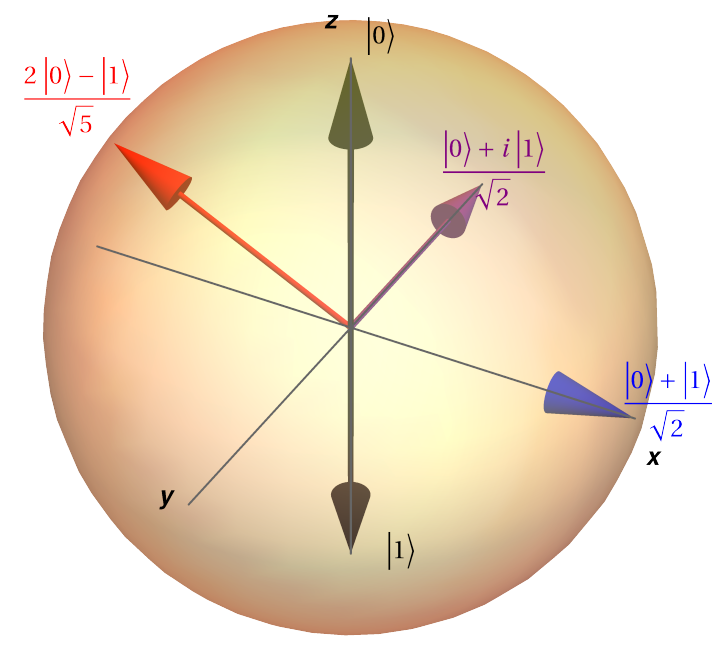
\includegraphics[width=5cm]
{img-congreso/bloch.png}
\end{minipage}
$\stackrel{\E_{z}\otimes\1 \vspace{1cm}}{\longmapsto}$
\begin{minipage}{0.4\textwidth}
\centering
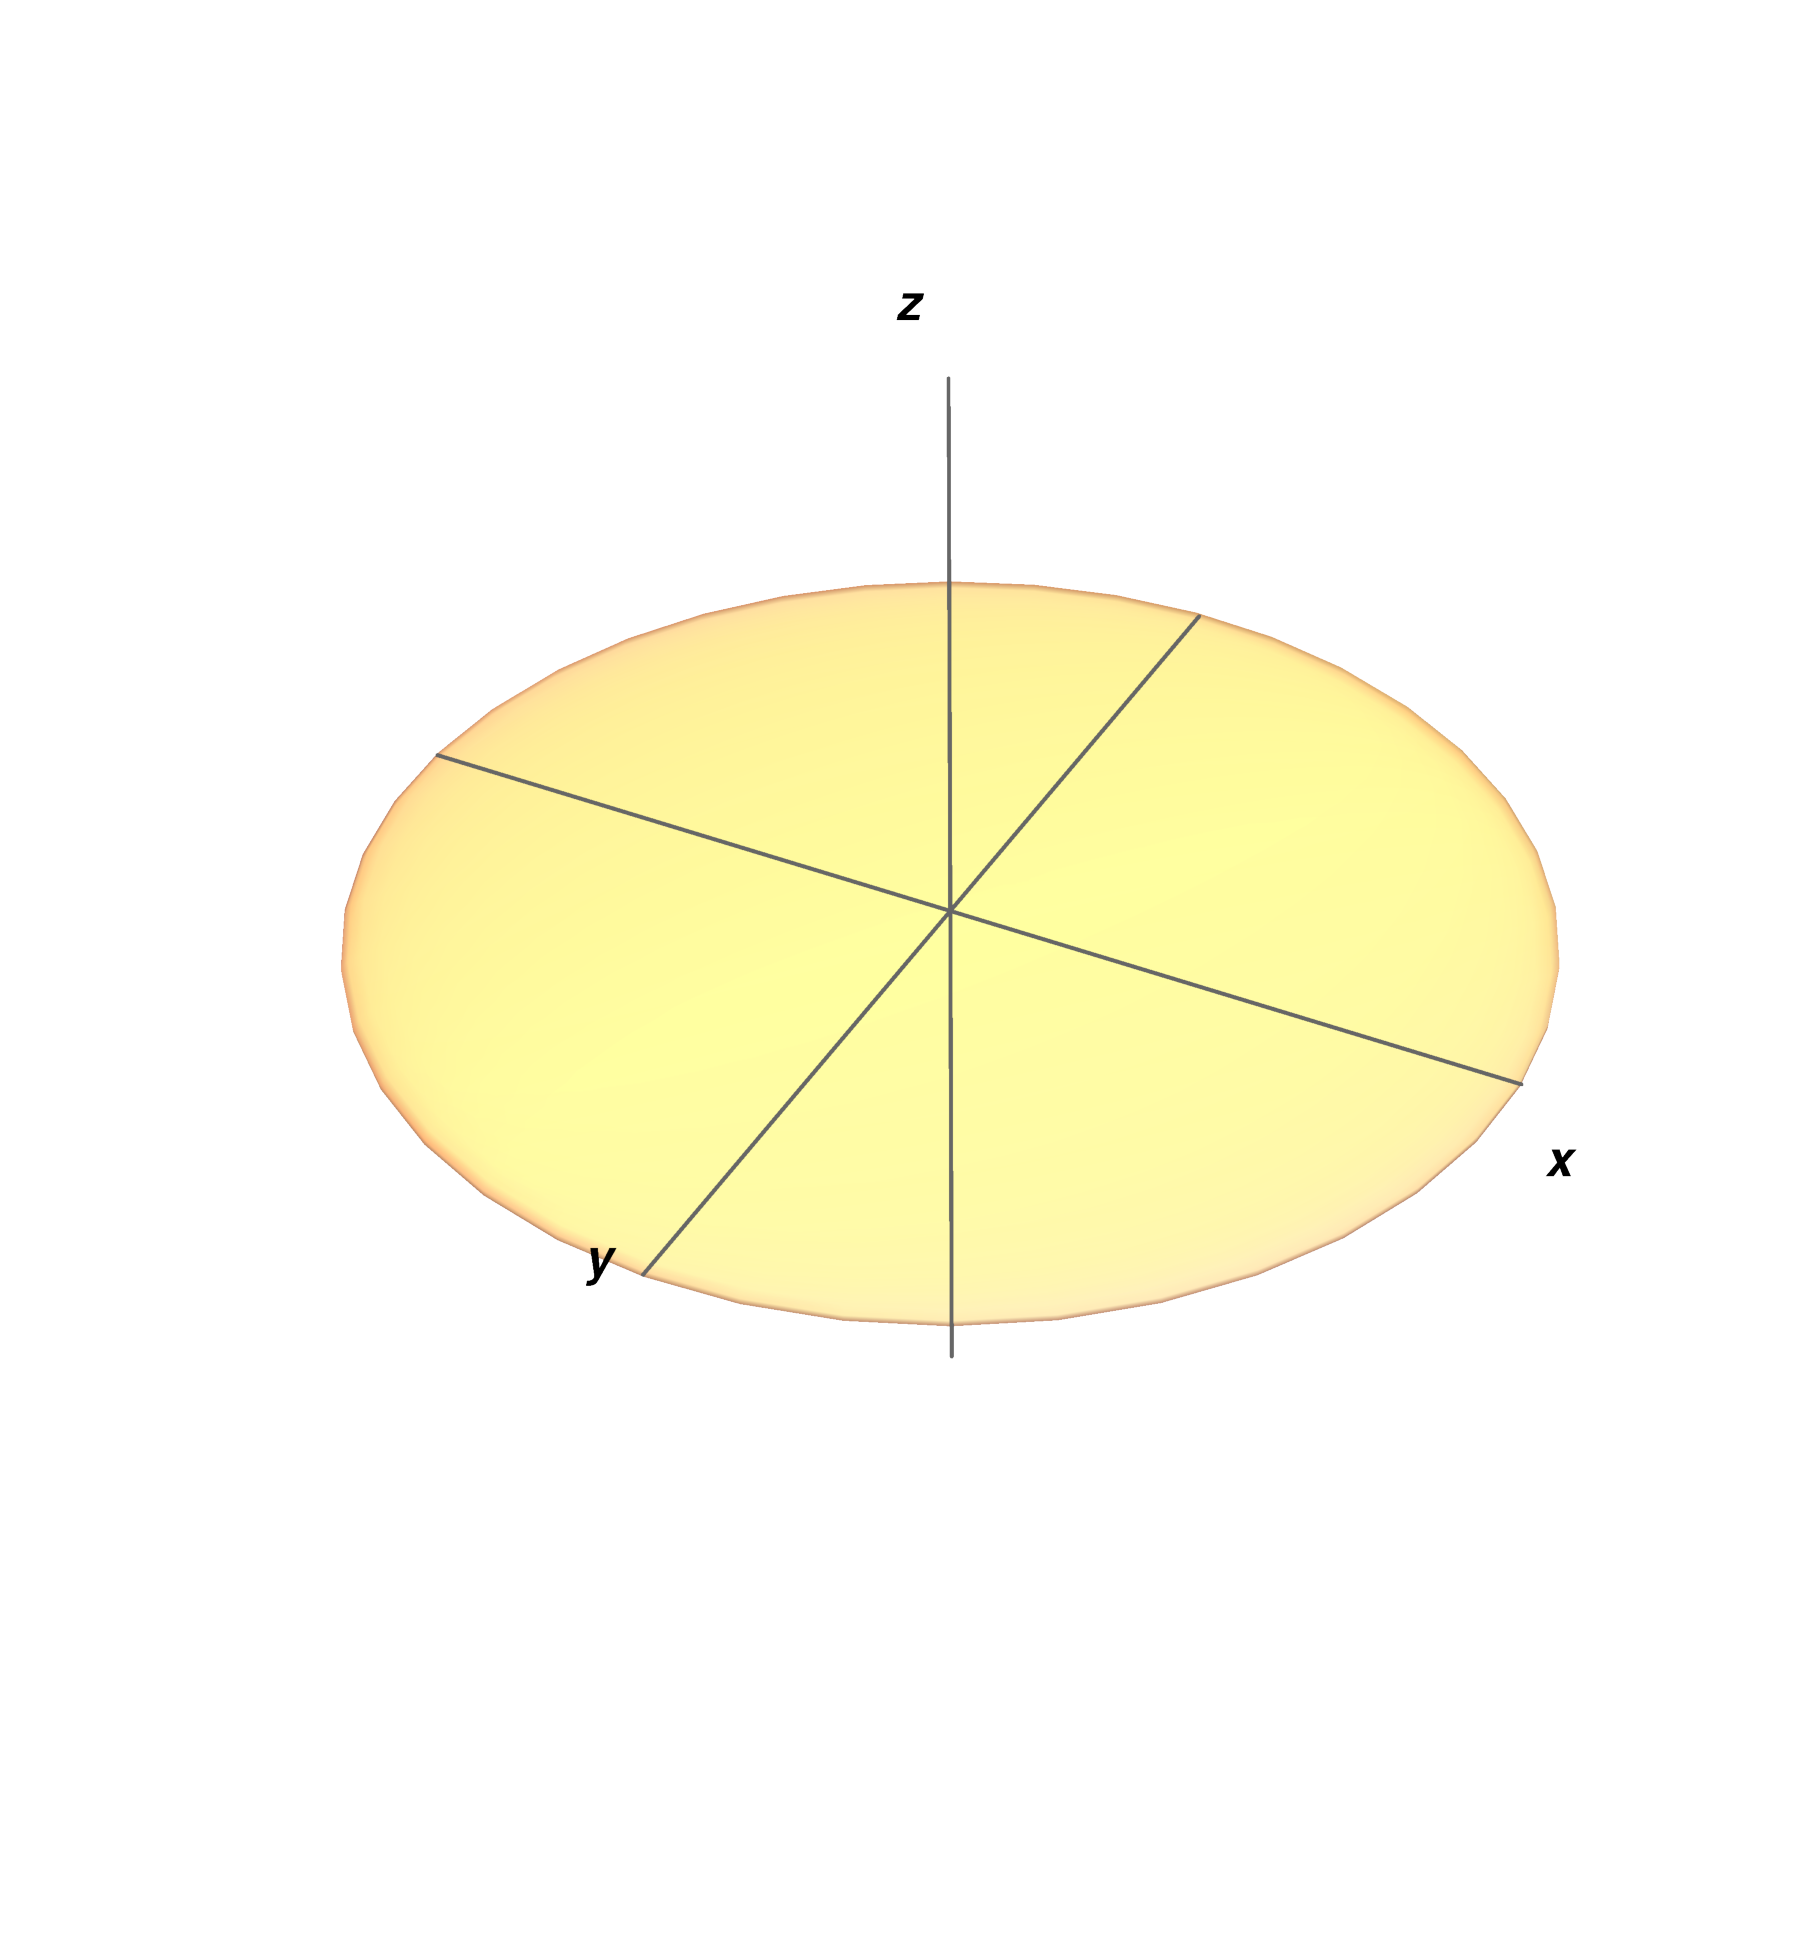
\includegraphics[width=6cm]
{img-congreso/DiskXY}
\end{minipage}
\caption{\cpnote{Prefuero dejar a las figuras realmente flotantes}
Deformación de la esfera de Bloch a un disco sobre el plano $XY$.}
\label{fig:qtm-op-motivation}
\end{figure} % }}}

Por otro lado, el estado máximamente entralazado $\rho^{\phi}$ de 
un sistema de 2 qubits es \cite{bengtsson_zyczkowski_2017}
\begin{align}
\rho^{\phi}&=
\mqty( 
\frac{1}{2} & 0 & 0 & \frac{1}{2} \\
0 & 0 & 0 & 0 \\
0 & 0 & 0 & 0 \\
\frac{1}{2} & 0 & 0 & \frac{1}{2} \\
).
\label{eq:DM-2q-MaxE}
\end{align}
De manera similar a \eqref{eq:DM-1q}, la matriz de densidad 
de 2 qubits se puede escribir como
\begin{align}
\rho&=\frac{1}{4}\sum _{i,j=0}^{3}r_{ij}\sigma_i\otimes\sigma_j,
\label{eq:DM-2q}
\end{align}
donde $\sigma_0=\1$ y $r$ es una matriz de $4\times4$ que contiene
la información física del sistema. Para encontrar $\rho^{\phi}$ en la
representación de \eqref{eq:DM-2q} se igualan 
\eqref{eq:DM-2q-MaxE} y \eqref{eq:DM-2q} y se resuelve
el sistema de ecuaciones para las componentes $r_{ij}$. De esa manera
se obtiene que $r_{00}=r_{11}=r_{33}=1$, $r_{22}=-1$, y el resto de 
entradas de $r$ son iguales a cero. 

Con $\rho^{\phi}$ en la representación de \eqref{eq:DM-2q} ahora
podemos estudiar la operación $\E_z\otimes\1$, la extensión 
de la operación $\E_z$ que actúa sobre los estados de 2 qubits. 
La operación $\E_z\otimes\1$ borra la componente en $z$ del 
qubit 1 y deja invariante el estado individual del qubit 2, 
es de decir que borra todos los elementos de la forma $r_{3j}$.
Por lo tanto, la matriz $r$ de $\rho^{\phi}$ bajo la acción de la 
operación $\E_z\otimes\1$ se transforma como
\begin{align}
r=
\mqty(
1&0&0&0\\
0&1&0&0\\
0&0&-1&0\\
0&0&0&1
)
\longmapsto
\mqty(
1&0&0&0\\
0&1&0&0\\
0&0&-1&0\\
0&0&0&0
)
=r'.
\end{align}
Con $r'$ determinado se calcula $\E_z\otimes\1\qty(\rho^{\phi})$ 
utilizando \eqref{eq:DM-2q} y se obtiene que el estado 
máximamente entrelazado $\rho^{\phi}$, bajo la acción de la
operación $\E_z\otimes\1$, se transforma como
\begin{align}
\mqty( 
\frac{1}{2} & 0 & 0 & \frac{1}{2} \\
0 & 0 & 0 & 0 \\
0 & 0 & 0 & 0 \\
\frac{1}{2} & 0 & 0 & \frac{1}{2} \\
)
\stackrel{\E_{z}\otimes\1}{\longmapsto}
\mqty( 
\frac{1}{4} & 0 & 0 & \frac{1}{2} \\
0 & \frac{1}{4} & 0 & 0 \\
0 & 0 & \frac{1}{4} & 0 \\
\frac{1}{2} & 0 & 0 & \frac{1}{4} \\
).
\end{align}
La matriz resultante $\E_z\otimes\1\qty(\rho^{\phi})$ tiene un 
autovalor igual a $-1/4$.
Por consiguiente, $\E_z\otimes\1\qty(\rho^{\phi})$ no es una matriz 
de densidad porque no es positiva.  
\cpnote{Se me hace bien el ejemplo, pero muy enredado el procedimiento. Quizá 
si lo platicamos, estaría bien.}
Dicho de otro modo, $\E_z\otimes\1\qty(\rho^{\phi})$ 
no describe a ningún estado físico de un sistema de 2 qubits.
En resumen, la operación $\E_z$ aunque transforma estados positivos
en estados positivos de 1 qubit, al considerar la extensión $\E_z\otimes\1$
aplicado sobre un estado particular de 2 qubits el resultado es un 
estado no válido. Por consiguiente, cualquier operación cuántica 
debe transformar estados positivos en estados positivos,
aún cuando el sistema principal interactúe con un sistema secundario,
sin importar la dimensión de este. El sistema secundario podría ser
el entorno, y es necesario que la condición de positividad de los estados
sea independiente de la dimensión del sistema secundario ya que 
en el laboratorio los grados de libertad del entorno son usualmente inaccesibles.
\cpnote{Esa ultima frase es blah blah. Mejorala}

De manera precisa, la definición de completa positividad es la siguiente.
Una operación $\E$ se dice que es completamente positiva (CP)
si y sólo si, para cualquier extensión dimensional arbitraria $K$ 
del espacio de Hilbert, tal que 
$\hi_N \rightarrow \hi_N \otimes \hi_K$,
el operador $\E\otimes\1_K$ es positivo semidefinido 
\cite{bengtsson_zyczkowski_2017}. 
\cpnote{No estoy seguro de que esa sea la definición. 
Mas bien, quieres decir que sea positivo}
Con esta definición, las condiciones 
que debe cumplir una operación cuántica para representar una evolución física 
están completas.

Una operación cuántica debe satisfacer dos condiciones: (1)
ser un mapeo afín de matrices de densidad, y (2) ser completamente positiva. 
En la literatura se suele utilizar el término operaciones 
cuánticas para operaciones CP que disminuyen la traza 
del operador de densidad, y el término canales cuánticos 
se restringe exclusivamente para operaciones CP
que preservan la traza del 
operador de densitad \cite{bengtsson_zyczkowski_2017}. 
A continuación, en las siguientes dos secciones discutiremos 
dos formas distintas de representar a las operaciones cuánticas.



%}}}
\section{Fomar de superoperador} % {{{
% \janote{\h{justificación:}
%     Propongo agregar esta sección por la línea de pensamiento que quiero seguir 
% durante todo el capítulo. Además porque numéricamente es 
% la representación que usamos\newline}
% \janote{
% Empezar hablando del reshape a $\rho$ (pasarlo de matriz a vector columna)
% \newline}
% \janote{Hablar de los mapeos que actúan sobre $\rho$ como un vector 
%     columna\newline}
% \janote{
%     Hablar de la matriz de Choi y enunciar el teorema de Choi: si la matriz
%  de Choi es positiva semidefinida entonces la operación cuántica es CP
%  \newline
% }
% \janote{
% Concluir con un ejemplo de un canal nuestro sobre 1 qubit
% \newline
% }
% \janote{Otro ejemplo, pero ahora sí de un canal \newline}

Una forma de representar a una operación cuántica es en la forma de 
superoperador. Un superoperador es una transformación lineal
que actúa sobre el espacio vectorial de los operadores lineales 
\cite{preskill1998lecture}. 
% \cpnote{Odio esas dos primeras frases}
Iniciaremos esta sección discutiendo algunas
transformaciones algebraicas sobre matrices e introduciremos 
una notación de cuatro índices que es útil al considerar un espacio de Hilbert 
compuesto por dos subsistemas. Luego vamos a presentar 
las condiciones que debe satisfacer un superoperador para ser un 
canal cuántico. Por último, vamos a presentar dos ejemplos de operaciones
lineales que actúan sobre la matriz de densidad de 1 qubit. En el primer 
ejemplo vamos a retomar la operación discutida en la sección anterior y, 
utilizando su forma de superoperador, vamos a mostrar que no es CP. 
Por último, en el segundo ejemplo discutiremos un canal cuántico
para familiarizar al lector con la forma de superoperador de un canal.

En la forma de superoperador de una operación cuántica se 
considera que la operación actúa sobre la matriz de densidad 
como un vector columna, por lo cual es necesario estudiar alguna transformación
lineal que reordene a una matriz en un vector columna, y viceversa.
Consideremos una matriz rectangular $A$ de dimensión $M\times N$.
La matriz puede reordenarse colocando sus elementos de matriz en 
orden lexicográfico en un vector $\vec{a}$ con $MN$ elementos, es decir
\begin{align}
a_k=A_{ij}, 
\label{eq:matrix-to-vector}
\end{align}
donde $k=\qty(i-1)N+j$, con $i=,1,\ldots,M$ y $j=1,\ldots,N$. De
esta manera, es posible reordenar a la matriz de densidad como un 
vector columna. Ante esta transformación los elementos de matriz no se 
modifican, por lo tanto la información física contenida en una matriz 
de densidad es invariante al vectorizarla.

Para determinar si una operación lineal, en su forma de superoperador, es CP 
se debe evaluar la positividad semidefinida de la matriz del superoperador
reordenada según un procedimiento conocido como \textit{reshuffle}.
La transformación de \textit{reshuffle} $R$ de una matriz cuadrada $B$ 
consiste en reordenar cada fila de $B$, con $MN$ elementos, 
en submatrices de dimensión $M\times N$ y colocarlas en 
orden lexicográfico bloque por bloque. Veamos un ejemplo del 
\textit{reshuffle} de una matriz $B$ de $4\times 4$, en la que 
cada fila se reordena en una submatriz de $2\times 2$
\begin{align}
B=
\mqty(
B_{00}&B_{01}&B_{02}&B_{03}\\
B_{10}&B_{11}&B_{12}&B_{13}\\
B_{20}&B_{21}&B_{22}&B_{23}\\
B_{30}&B_{31}&B_{32}&B_{33})
\stackrel{R}{\longrightarrow}
\mqty(
B_{00}&B_{01}&B_{10}&B_{11}\\
B_{02}&B_{03}&B_{12}&B_{13}\\
B_{20}&B_{21}&B_{30}&B_{31}\\
B_{22}&B_{23}&B_{32}&B_{33})
=B^R.
\label{eq:reshuffle}
\end{align}
Más adelante veremos que la matriz del superoperador 
reordenada mediante el \textit{reshuffle} se define como la matriz de Choi
de la operación.

Para establecer las condiciones que una operación, en su
forma de superoperador, debe cumplir para ser un mapeo afín de
matrices de densidad es útil introducir la siguiente notación de cuatro índices. 
Supongamos que $U$ es un operador que actúa sobre un espacio de Hilbert 
compuesto de la forma $\hi=\hi_M\otimes\hi_N$.
Sea $\ket{i}$ una base ortonormal de $\hi_M$ y $\ket{\mu}$ una base
ortonormal de $\hi_N$. Nótese el uso de letras latinas para los índices del
primer subsistema y letras griegas para los índices del segundo.
El producto tensorial $\ket{i}\otimes\ket{\mu}$
es una base del espacio compuesto $\hi$. Por lo tanto, un 
elemento de matriz de $U$, utilizando cuatro índices, es
\begin{align}
U_\ind{m\mu}{n\nu}=\matrixel{i\otimes \mu}{U}{j\otimes \nu}.
\label{eq:4indices}
\end{align}

Hasta ahora lo que hemos expuesto nos permite reordenar a una matriz
de densidad $\rho$ de dimensión $N\times N$ en un vector con $N^2$ 
elementos. Por consiguiente, la matriz $\E$, en su forma de 
superoperador que actúa sobre una matriz de densidad vectorizada $\vec{\rho}$, 
debe ser de dimensión $N^2\times N^2$. Los elementos de matriz de
$\E$ pueden etiquetarse utilizando cuatro índices como en \eqref{eq:4indices},
haciendo cualquier partición en dos del sistema de Hilbert total.

Una operación $\E$ que sea candidata a canal cuántico debe transformar 
matrices de densidad en matrices de densidad. Esto quiere decir que
la imagen $\rho'$, de una matriz de densidad $\rho$, debe ser (i) Hermítica, 
(ii) de traza unitaria y (iii) positiva semidefinida. 
Cada una de estas condiciones sobre $\rho'$ impone una condición 
sobre el superoperador $\E$ \cite{bengtsson_zyczkowski_2017}:
\begin{align}
\txt{(i)}&& \rho'=\qty(\rho')^{\dagger}&&\Leftrightarrow
    && \E_\ind{m\mu}{n\nu}=\E_\ind{\mu m}{\nu n}^*,&&
    \label{eq:H-condition}\\
\txt{(ii)}&&\Tr(\rho')=1
    &&\Leftrightarrow&&  \E_\ind{mm}{n\nu}=\delta_{n\nu},\\     
\txt{(iii)}&&\rho'\geq1
    &&\Leftrightarrow&&  \E_\ind{m\mu}{n\nu}\rho_{n\nu}\geq0.
    \label{eq:positivity-condition}
\end{align}

Según lo que discutimos en la sección anterior estas condiciones
no son suficientes para que la operación $\E$ sea un canal cuántico; adicionalmente 
$\E$ debe ser CP. Para evaluar la completa positividad de $\E$, en su forma 
de superoperador, vamos a definir a la matriz de Choi $D_{\E}$ como 
\cite{bengtsson_zyczkowski_2017}
\begin{align}
D_{\E}=\E^{R}.
\end{align}
Es decir, la matriz de Choi de $\E$ es la matriz que resulta del \textit{reshuffle}
de la matriz del superoperador $\E$. 
Con la matriz de Choi $D_{\E}$ definida vamos a enunciar 
el teorema de Choi \cite{bengtsson_zyczkowski_2017} que
establece si $\E$ es CP evaluando la positividad semidefinida de $D_{\E}$.
\begin{teorema}
Una transformación lineal $\E$ es completamente positiva si y sólo si 
su matriz de Choi asociada $D_{\E}$ es positiva semidefinida.
\end{teorema}
Este teorema completa las herramientas para establecer el procedimiento 
para evaluar si $\E$ como superoperador es un canal cuántico. 
Dado que una operación $\E$ cumple con las condiciones establecidas de
\eqref{eq:H-condition} a \eqref{eq:positivity-condition}, la positividad
de la matriz de Choi $D_{\E}$ determina si la operación es 
o no un canal cuántico.

Ahora retomemos el ejemplo de la operación $\E_z$ 
sobre 1 qubit de la sección anterior para evaluar la condición de 
completa positividad de la operación en su forma de superoperador. 
Recordemos que la acción de $\E_z$ sobre la 
esfera de Bloch se ilustra en la \Fref{fig:qtm-op-motivation}.
La expresión \eqref{eq:notCP} especifica el vector de Bloch
de la matriz de densidad $\rho'$, imagen de $\rho$ bajo la acción de $\E_z$.
Por lo tanto, al vectorizar $\rho$ y $\rho'$ el cálculo 
de la matriz de superoperador $\E_z$ es directo. 
De esa manera, la ecuación de transformación 
de la matriz de densidad $\rho$ de un qubit, bajo la
acción de la operación $\E_z$ en su forma de superoperador, es
\begin{align}
\mqty(
\frac{1}{2} & 0 & 0 & \frac{1}{2} \\
0 & 1 & 0 & 0 \\
0 & 0 & 1 & 0 \\
\frac{1}{2} & 0 & 0 & \frac{1}{2} \\
)
\frac{1}{2}
\mqty(
1+r_z\\r_x-ir_y\\r_x+ir_y\\1-r_z
)
=
\frac{1}{2}
\mqty(
1\\r_x-ir_y\\r_x+ir_y\\1
).
\end{align}
Se aplica el procedimiento de \textit{reshuffle} a la matriz en la ecuación 
anterior y se obtiene que la matriz de Choi de la operación $\E_z$ es
\begin{align}
\E_z^R=
\mqty(
\frac{1}{2} & 0 & 0 & 1 \\
0 & \frac{1}{2} & 0 & 0 \\
0 & 0 & \frac{1}{2} & 0 \\
1 & 0 & 0 & \frac{1}{2} 
).
\end{align}
La matriz $\E_z^R$ tiene un autovalor $-1/2$, 
por consiguiente $\E_z$ no es CP. 
En la forma de superoperador de $\E_z$ hemos llegado a la misma
conclusión de la sección anterior sobre la 
completa positividad.

Para concluir la sección será útil desarrollar un ejemplo más, 
pero ahora de una operación que sí es un canal cuántico de 1 qubit. Este 
ejemplo servirá para proporcionar más familiaridad con la forma de 
los superoperador y, además, para hacer la conexión con 
la forma de Kraus de las operaciones cuánticas en la siguiente sección.

\begin{figure} % {{{
    \centering
    \begin{minipage}{.4\textwidth}
        \centering
        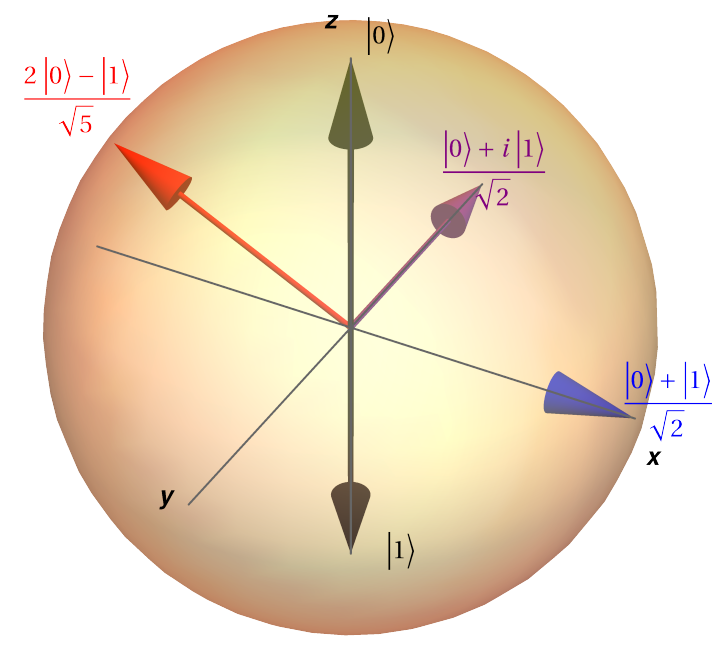
\includegraphics[width=5cm]
        {img-congreso/bloch.png}
    \end{minipage}
    $\stackrel{\E_{xz}\otimes\1 \vspace{1cm}}{\longmapsto}$
    \begin{minipage}{0.4\textwidth}
        \centering
        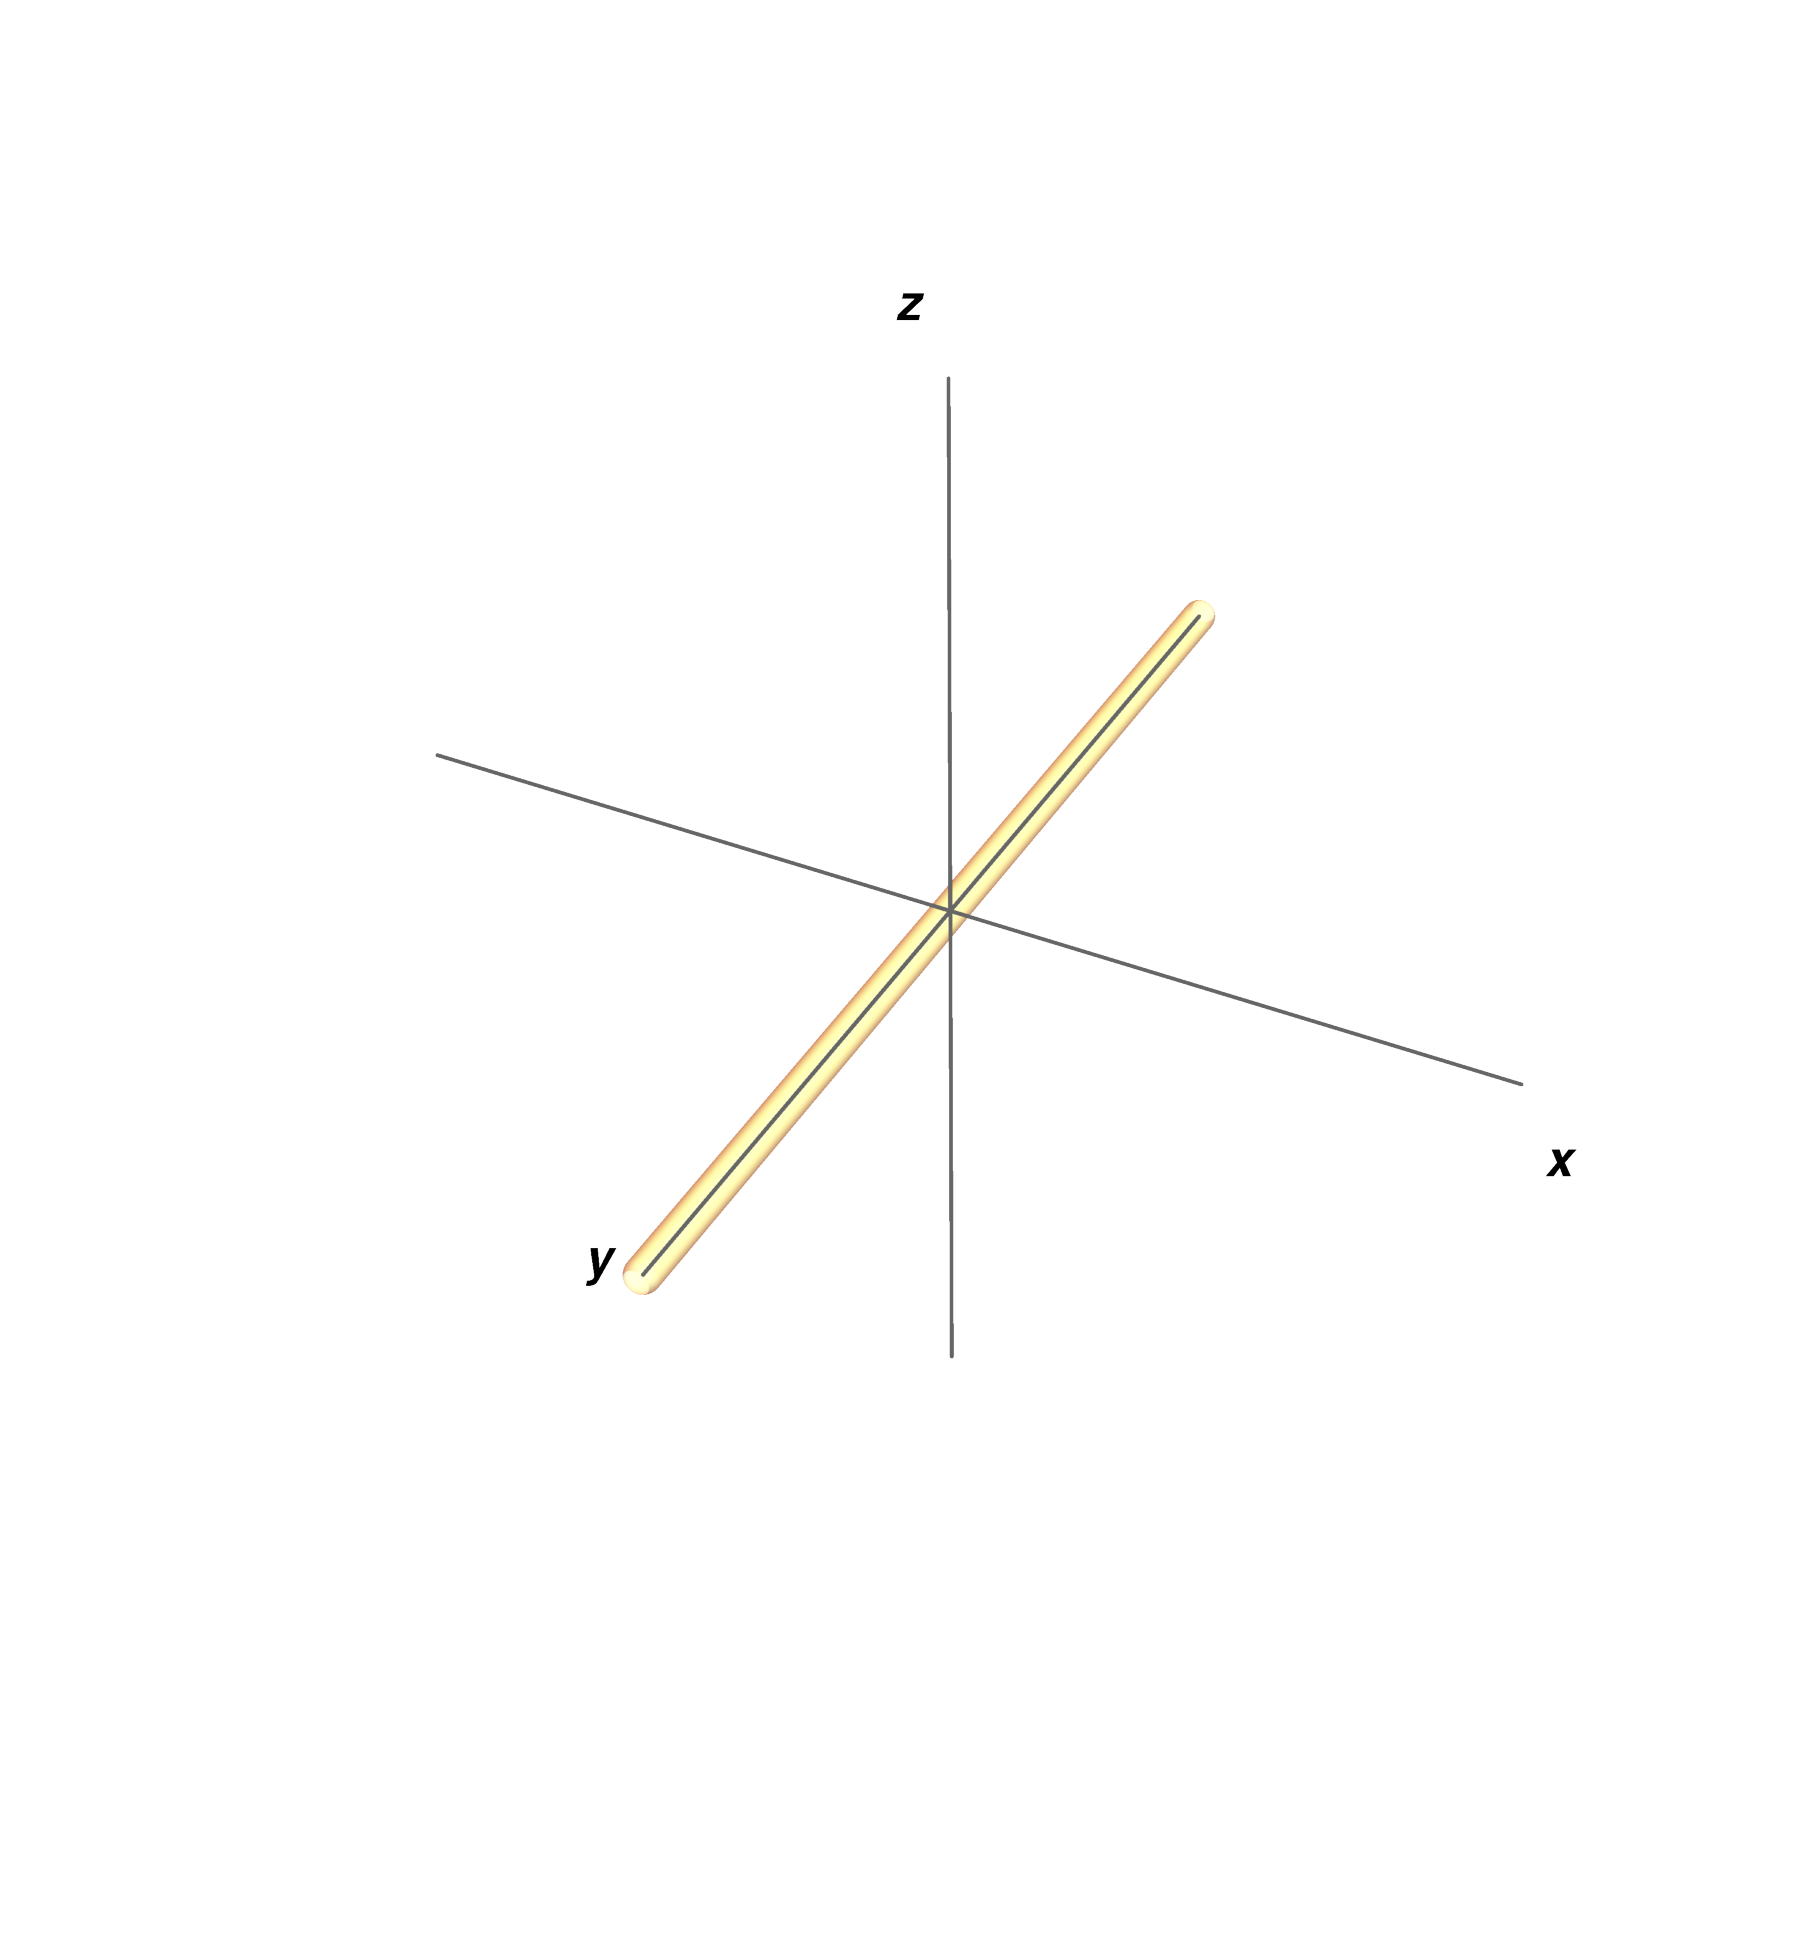
\includegraphics[width=6cm]
        {img-congreso/lineY}
    \end{minipage}
    \caption{Deformación de la esfera de Bloch a un disco sobre el plano $XY$.}
    \label{fig:QC-ex2}
\end{figure} % }}}
Consideremos la operación $\E_{xz}$ que colapsa la esfera de Bloch
al eje $y$ como se muestra en la \Fref{fig:QC-ex2}. El vector de 
Bloch de cualquier punto en la esfera se proyecta hacia el eje $y$.
A partir de la representación geométrica de $\E_{xz}$ 
se puede inferir que el vector de Bloch se transforma 
como
\begin{align}
\qty(r_x,r_y,r_z)\mapsto\qty(0,r_y,0),
\label{eq:Bloch-vec-mapToY}
\end{align}
con lo cual se determina $\rho'$ y, seguidamente,
la matriz del superoperador $\E_{xz}$.
Por lo tanto, la ecuación de transformación de la matriz 
de densidad de 1 qubit, bajo la acción de $\E_{xz}$ y 
en su forma de superoperador, es
\begin{align}
\mqty(
\begin{array}{cccc}
\frac{1}{2} & 0 & 0 & \frac{1}{2} \\
0 & \frac{1}{2} & -\frac{1}{2} & 0 \\
0 & -\frac{1}{2} & \frac{1}{2} & 0 \\
\frac{1}{2} & 0 & 0 & \frac{1}{2} \\
\end{array}
)
\frac{1}{2}
\mqty(
1+r_z\\r_x-ir_y\\r_x+ir_y\\1-r_z
)
=
\frac{1}{2}
\mqty(
1\\-ir_y\\ir_y\\1
).
\label{eq:QC-ex2-SR}
\end{align}
Al calcular la matriz de Choi de la operación notamos 
que $\E_{xz}=\E_{xz}^R$ e, inmediatamente, se concluye
que $\E_{xz}$ es completamente positiva. La operación $\E_{xz}$
es un canal cuántico.

En resumen, en la forma de superoperador de una operación cuántica $\E$
se considera a $\E$ como una matriz que actúa sobre 
una matriz de densidad vectorizada $\vec{\rho}$. 
Si una operación $\E$ satisface las condiciones de
\eqref{eq:H-condition} a \eqref{eq:positivity-condition}, entonces
es un mapeo afín de matrices de densidad.
Además, el procedimiento de \textit{reshuffle} 
proporciona una manera para calcular la matriz de Choi de
 $\E$; y, según el teorema de Choi, si 
la matriz de Choi es positiva semidefinida, entonces $\E$ es 
completamente positiva. 
Así, hemos establecido las herramientas y condiciones para evaluar 
si una operación en su forma de superoperador es un canal cuántico.
En la siguiente sección presentaremos la forma de Kraus de las operaciones
cuánticas.

%}}}
\section{Forma de Kraus} % {{{
\janote{
- Enunciar la representación en operadores de suma partiendo de un 
estado que se acopla con algún entorno
y llegar a las condiciones para ser CPTP y empezar a conectarlo
con la sección anterior.} \cpnote{No sabes si hay alguna motivacion que no sea
con el entorno? Realmente no lo usamos y se me hace meter una complicación adicional}
\janote{Entonces voy a omitir la motivación con el entorno y en general
    mencionar al entorno en la explicación.\newline}
\janote{Introducción\newline}
\janote{
    - Invocar el ejemplo del canal de la sección anterior, pero en su 
    representación de operadores de suma. Aquí quiero hacer la conexión 
    entre esta y la sección anterior mostrando que los operadores 
    de Kraus son los autovectores de la matriz de Choi.\newline}
\janote{
    - Comparar la representacion de suma de operadores y superoperadores
\newline}

Otra forma de representar a una operación cuántica, distinta a la
forma de superoperador de la sección anterior, es la forma de Kraus. 
La diferencia principal entre ambas representaciones 
es que la forma de superoperador
representa a una operación cuántica como una matriz que 
actúa sobre el espacio de los operadores lineales, por otro lado,
la forma de Kraus representa a una operación cuántica 
como operadores que actúan sobre el espacio de 
Hilbert del sistema. Vamos a iniciar retomando el segundo 
ejemplo de la sección anterior, en el cual estudiamos 
el canal cuántico $\E_{xz}$, cuya acción sobre la esfera
de Bloch se muestra en la \Fref{fig:QC-ex2}.
Luego vamos a mostrar cómo encontrar la forma de Kraus de $\E_{xz}$ 
a partir de la forma de superoperador del canal.
Para terminar, se presentarán las condiciones 
que debe cumplir una operación en la forma de Kraus para
ser un canal cuántico.

Consideremos de nuevo el canal cuántico $\E_{xz}$.
Recordemos que $\E_{xz}$ es un canal cuántico
que colapsa la esfera de Bloch al eje $y$. 
Vamos a calcular los autovectores y autovalores de la 
matriz de Choi, luego al reordenar
cada autovector como matriz y multiplicarlo por la raíz cuadrada
del autovalor correspondiente obtendremos los llamados 
operadores de Kraus; después, al operarlos con la matriz 
de densidad de 1 qubit, según 
la forma de Kraus, mostraremos que se obtiene el 
resultado de la ecuación \eqref{eq:QC-ex2-SR}.

Recordemos que la matriz de la ecuación \eqref{eq:QC-ex2-SR}
es la matriz del superoperador de $\E_{xz}$ y, al mismo tiempo,
la matriz de Choi del canal $(\E_{xz}=\E_{xz}^R)$.  
Se calculan los autovectores $\ket{E_{1,2,3,4}}$ de 
la matriz de Choi y se obtienen
\begin{align}
\ket{E_{1,2,3,4}}=
\mqty(\frac{1}{2},0,0,\frac{1}{2})^T,
\mqty(0,-\frac{1}{2},\frac{1}{2},0)^T,
\mqty(-\frac{1}{2},0,0,\frac{1}{2})^T,
\mqty(0,\frac{1}{2},\frac{1}{2},0)^T,
\end{align}
cuyos autovalores son $\lambda_{1,2,3,4}=1/2,1/2,0,0$, respectivamente.
Se reordena cada autovector $\ket{E_i}$ en una matriz
$E_i$ de $2\times2$, siguiendo el procedimiento 
inverso de vectorización establecido en
\eqref{eq:matrix-to-vector}, y luego se multiplica cada $E_i$ por 
la raíz cuadrada de su autovalor respectivo. Se obtiene
\begin{align}
E_1&=
\frac{1}{\sqrt{2}}
\mqty(
1 & 0\\
0 & 1
),
&
E_2&=
\frac{1}{\sqrt{2}}
\mqty(
0 & -1\\
1 & 0
).
\end{align}
Ahora operamos a la matriz de densidad de 1 qubit 
\eqref{eq:DM-1q} siguiendo la operación
\begin{align}
\rho'=\sum_{i=1}^2E_i\rho E_i^{\dagger}
\label{eq:Kraus}
\end{align}
que se conoce como la forma de Kraus de una operación cuántica. Operando
\begin{align}
\rho'=&
\frac{1}{2}
\mqty(
1 & 0\\
0 & 1
)
\mqty(
\frac{1+r_z}{2}& \frac{r_x-ir_y}{2}\\
\frac{r_x+ir_y}{2} & \frac{1-r_z}{2}
)
\mqty(
1 & 0\\
0 & 1
)
+
\frac{1}{2}
\mqty(
0 & -1\\
1 & 0
)
\mqty(
\frac{1+r_z}{2}& \frac{r_x-ir_y}{2}\\
\frac{r_x+ir_y}{2} & \frac{1-r_z}{2}
)
\mqty(
0 & 1\\
-1 & 0
)&
\nonumber\\
\rho'=&
\frac{1}{2}
\mqty(
1 & -ir_y\\
ir_y & 1
).
\label{eq:QC-ex2-KR}
\end{align}
Hemos obtenido el mismo resultado de la ecuación 
\eqref{eq:QC-ex2-SR}, pero reordenado como matriz. 
No obstante, los operadores $E_i$ son
operadores que también actúan sobre el espacio de Hilbert de 1 qubit. 
La ecuación \eqref{eq:Kraus} se conoce 
como la forma de \textit{Kraus} de los mapeos completamente positivos
\cite{bengtsson_zyczkowski_2017}.
Los autovectores de la matriz de Choi de una operación cuántica $\E$,
reordenados como matrices, se
reciben el nombre de operadores de Kraus $E_i$ de la operación cuántica.
Los operadores $E_i$ linealmente independientes  
pueden ser hasta $N^2$ \cite{nielsen_chuang_2011}, igual a la dimensión 
del espacio de los operadores lineales que actúan sobre un espacio de
Hilbert de dimensión $N$. 
Finalmente, una operación cuántica $\E$ preserva la traza de la matriz de densidad 
si y sólo sus operadores de Kraus $E_i$ satisfacen la condición
\cite{bengtsson_zyczkowski_2017}
\begin{align}
\sum_iE_i^{\dagger}E_i=\1.
\label{eq:kraus-tp-cond}
\end{align}

En resumen, las ecuaciones \eqref{eq:Kraus} y \eqref{eq:kraus-tp-cond}
caracterizan la forma de Kraus de un canal cuántico. 
Con esto hemos mostrado dos formas distintas de representar a un 
canal cuántico: la forma de superoperador, una matriz cuadrada
de dimensión $N^2$, que actúa sobre una matriz de densidad vectorizada 
con $N^2$ entradas; y la forma de Kraus, matrices que actúan sobre
una matriz de densidad que también pertenecen al espacio de 
los operadores lineales que actúan sobre el espacio de Hilbert. La matriz de 
Choi de un canal cuántico proporciona una manera de conectar ambas 
representaciones. Por un lado, si $D_{\E}$ es la matriz de Choi de un canal 
cuántico $\E$, entonces $D_{\E}^R$ es la matriz de superoperador
del canal.
Por otro lado, los autovectores de $D_{\E}$,
multiplicados por la raíz cuadrada de sus autovalores asociados,
son los operadores de Kraus del canal cuántico. 

%}}}
\section{Canales cuánticos de 1 qubit} % {{{
\janote{
- Hablar de que se gana intuición pensando en la acción de un canal de 1
qubit como la manera en que deforma la esfera de Bloch\newline}
\janote{
- Ejemplos: phase-flip channel, depolarizing y amplitude damping\newline}

Mostrar algunos ejemplos de canales cuánticos de 1 qubit 
puede proporcionar intuición 
para completar el marco teórico de los canales cuánticos. 
Como se presentó en los ejemplos que abordamos en las 
secciones anteriores, para los sistemas de 1 qubit se tiene la
herramienta geométrica de la esfera de Bloch para asociar cada 
punto de ella con un estado del sistema. De esa manera, 
se puede visualizar la acción de un canal cuántico como la 
deformación de la esfera de Bloch bajo la acción del canal.
En esta sección vamos a estudiar la acción de tres canales 
cuánticos representativos de 1 qubit, presentaremos
la forma de superoperador, así como la forma de Kraus de 
cada uno de los canales cuánticos.

El canal inversor de fase y bit $\E_{BPF}$ intercambia 
los estados $\ket{0}$ y $\ket{1}$, 
autoestados de $\sigma_z$, e intercambia la fase total
del estado $\ket{\psi}$ de un qubit con probabilidad $1-p$. 
Recordemos que el vector $\vec{r}$ de la matriz de densidad en \eqref{eq:DM-1q} 
especifica las coordenadas $r_i$ en la esfera de Bloch del punto asociado al estado
en el que se encuentra el sistema. La acción de $\E_{BPF}$ es 
equivalente a la siguiente transformación del vector de Bloch $\vec{r}$
\begin{align}
\qty(r_x,r_y,r_z)\rightarrow&\Big(\qty(1-2p)r_x,r_y,\qty(1-2p)r_z\Big).
\label{eq:bit-phase-flip-Bloch-trans}
\end{align}
Geométricamente, el vector de Bloch es proyectado por $\E_{BPF}$ 
al eje $y$ y las componentes en $x$ y $z$ se pierden, como 
se muestra en la \Fref{fig:bit-phase-flip}.
Notemos que el ejemplo que discutimos en la sección 2.2 del 
canal cuántico que colapsa la esfera de Bloch al eje $y$ es un caso
particular de $\E_{BPF}$ cuando $p=0.5$.
\begin{figure}[H]
\centering
\begin{minipage}{.4\textwidth}
    \centering
    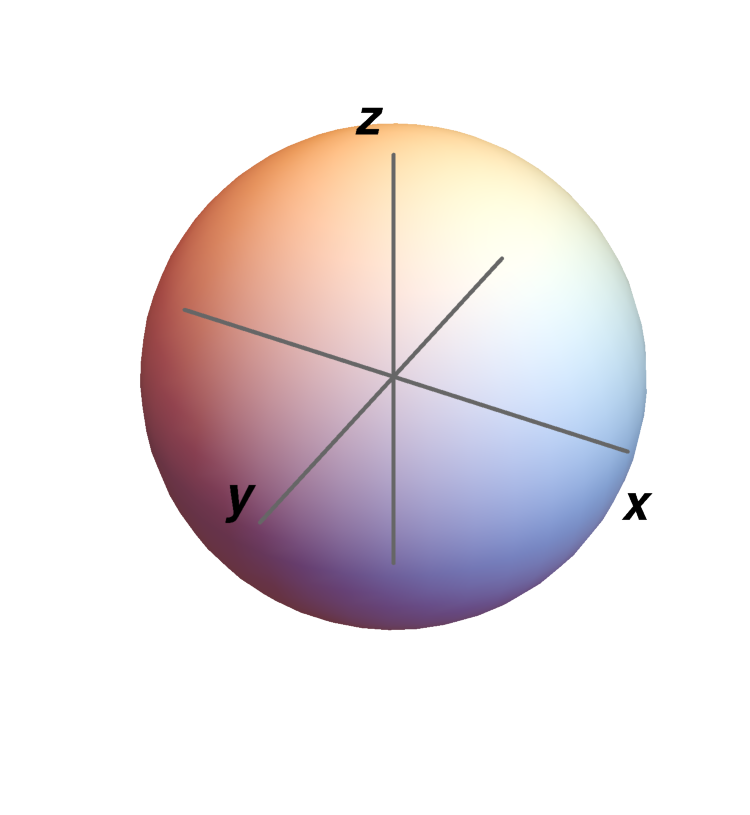
\includegraphics[width=6cm]{images/bloch-ball}
\end{minipage}
$\longmapsto$
\begin{minipage}{0.4\textwidth}
    \centering
    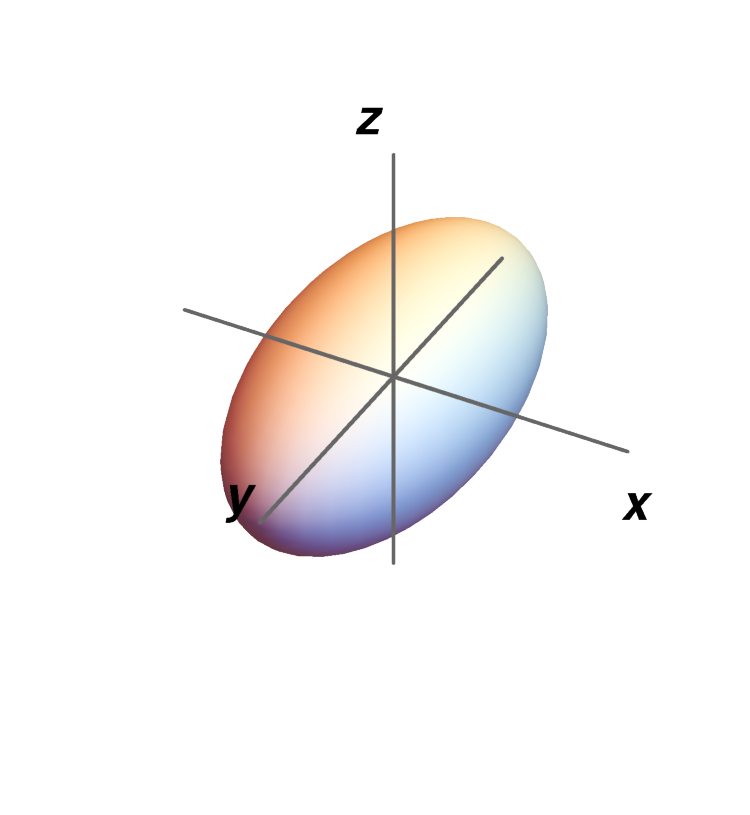
\includegraphics[width=6cm]{images/bit-phase-flip}
\end{minipage}
\caption{Efecto del canal inversor de fase y bit sobre la esfera de Bloch, 
para $p=0.3$.}
\label{fig:bit-phase-flip}
\end{figure}
La expresión en \eqref{eq:bit-phase-flip-Bloch-trans} nos 
permite calcular la matriz de densidad $\rho'$ que resulta
bajo la acción del canal inversor de fase y bit. Por lo tanto, 
vectorizando $\rho$, $\rho'$ y aplicando métodos elementales de
álgebra lineal para calcular la matriz del superoperador
se encuentra que la ecuación de transformación de
la matriz de densidad de 1 qubit bajo la acción 
de $\E_{BPF}$ es
\begin{align}
\frac{1}{2}
\mqty(
1-p & 0 & 0 & p \\
0 & 1-p & -p & 0 \\
0 & -p & 1-p & 0 \\
p & 0 & 0 & 1-p \\
)
\frac{1}{2}
\mqty(
1+r_z\\r_x-ir_y\\r_x+ir_y\\1-r_z
)
=
\frac{1}{2}
\mqty(
1+\qty(1-p)z\\
\qty(1-p)x-i y\\
\qty(1-p)x+i y\\
1-\qty(1-p)z
).
\label{eq:bpf-supero}
\end{align}
Para encontrar los operadores de Kraus se determinan los autovectores
de la matriz de Choi $D_{\E_{BPF}}$ del canal inversor de fase y bit. 
Para encontrar la matriz de Choi se aplica la transformación 
de \textit{reshuffle} a la matriz en la ecuación \eqref{eq:bpf-supero}.
Los autovectores de $D_{\E_{BPF}}$, reordenados como matrices y
cada uno multiplicado por la raíz cuadrada de su autovalor respectivo, son
\begin{align}
E_0&=
\sqrt{p}
\mqty(
1 & 0\\
0 & 1
)&
E_1&=
\sqrt{1-p}
\mqty(
0 & -1\\
1 & 0
).
\label{eq:bpf-kraus}
\end{align}
Así hemos encontrado la forma de superoperador y de Kraus del canal
cuántico inversor de fase y bit $\E_{BPF}$. Se puede evaluar directamente que 
tanto la matriz en \eqref{eq:bpf-supero} como los operadores $E_i$
en \eqref{eq:bpf-kraus} cumplen con las condiciones respectivas
para ser canales cuánticos.

Ahora estudiaremos el canal depolarizante $\E_{Dep}$, que se muestra
en la \Fref{fig:depolarizing}, cuya acción sobre el 
vector de Bloch con probabilidad $(1-p)$ es 
\begin{align}
\qty(r_x,r_y,r_z)\rightarrow&\Big(\qty(1-p)r_x,\qty(1-p)r_y,\qty(1-p)r_z\Big).
\label{eq:depolarizing-bloch-vec}
\end{align}
Geométricamente, el canal $\E_{Dep}$ atenúa por igual todas las 
componentes del vector de Bloch y tiene como caso límite $(p=1)$
el mapeo de cualquier estado de 1 qubit al estado 
de máxima ignorancia o máximamente mixto $\1/2$
\cite{bengtsson_zyczkowski_2017}, asociado con el origen de coordenadas.
\begin{figure}[H]
    \centering
    \begin{minipage}{.4\textwidth}
        \centering
        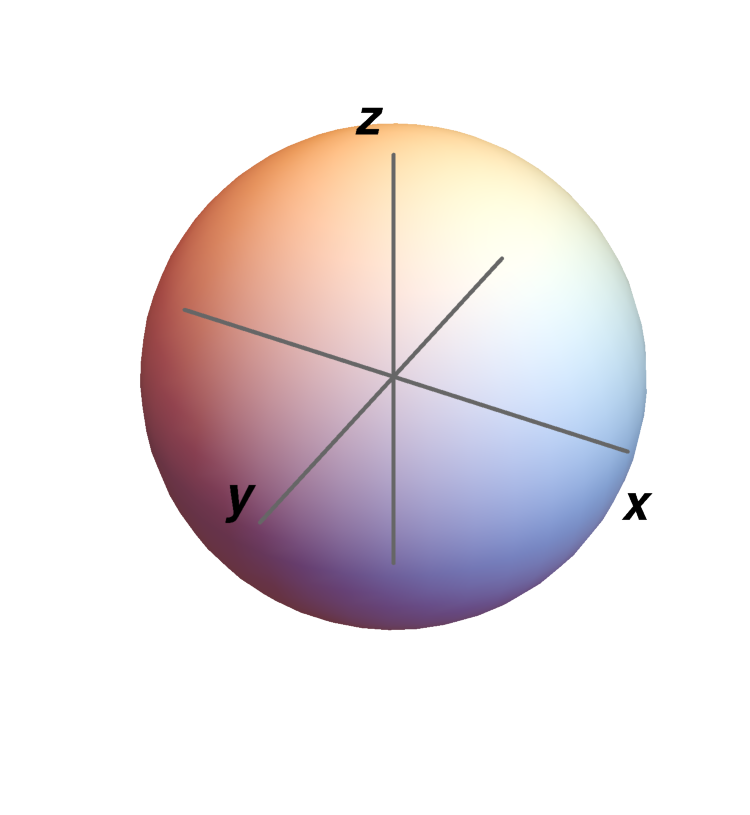
\includegraphics[width=6cm]{images/bloch-ball}
    \end{minipage}
    $\longmapsto$
    \begin{minipage}{0.4\textwidth}
        \centering
        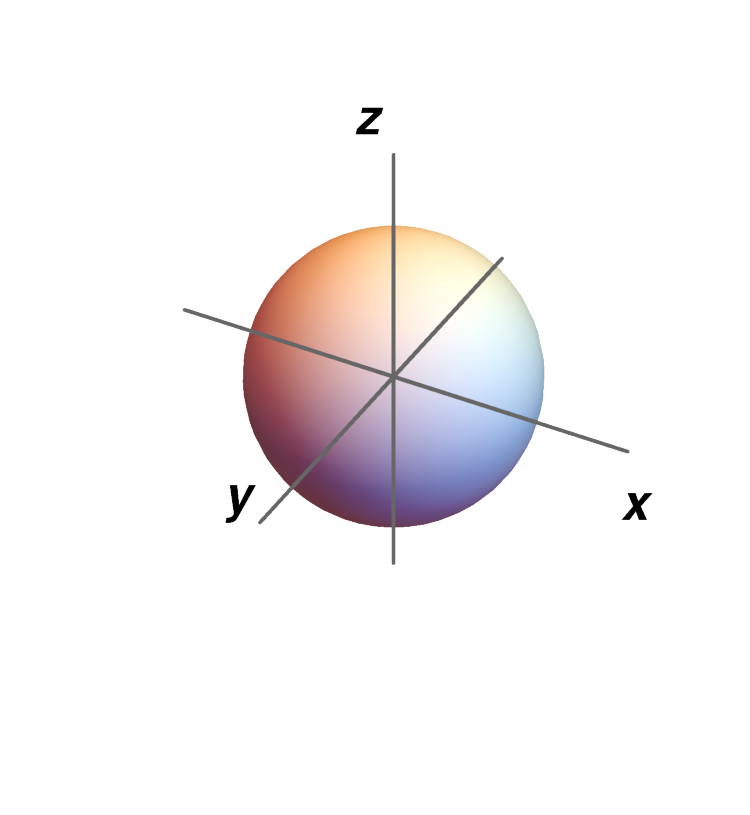
\includegraphics[width=6cm]{images/depolarizing}
    \end{minipage}
    \caption{Efecto del canal depolarizante sobre la esfera de Bloch, 
    para $p=0.4$.}
    \label{fig:depolarizing}
\end{figure}
Repitiendo el procedimiento del ejemplo anterior para calcular 
la ecuación de transformación de la matriz de densidad de
1 qubit bajo la acción de $\E_{Dep}$ en su forma de 
superoperador se encuentra que es
\begin{align}
\frac{1}{2}
\mqty(
1-\frac{p}{2} & 0 & 0 & \frac{p}{2} \\
0 & 1-p & 0 & 0 \\
0 & 0 & 1-p & 0 \\
\frac{p}{2} & 0 & 0 & 1-\frac{p}{2}
)
\frac{1}{2}
\mqty(
1+r_z\\r_x-ir_y\\r_x+ir_y\\1-r_z
)
=
\frac{1}{2}
\mqty(
1+\qty(1-p)z\\
\qty(1-p)\qty(x-i y)\\
\qty(1-p)\qty(x+i y)\\
1-\qty(1-p)z
),
\end{align}
y calculando los autovectores y autovalores de la matriz de Choi de
$\E_{Dep}$ se encuentra que los operadores de Kraus del 
canal depolarizante son
\begin{align}
E_0&=
\sqrt{1-\frac{3p}{4}}
\mqty(
1 & 0\\
0 & 1
),&
E_1&=
\frac{\sqrt{p}}{2}
\mqty(
-1 & 0\\
0 & 1
),\\
E_2&=
\frac{\sqrt{p}}{2}
\mqty(
0 & -1\\
1 & 0
), &
E_3&=
\frac{\sqrt{p}}{2}
\mqty(
0 & 1\\
1 & 0
).
\end{align}
Los dos ejemplos anteriores son canales cuánticos que dejan invariantes 
el estado máximamente mixto. Es decir, $\E(\1/2)=\1/2$. Los canales que
satisfacen esta condición se conocen como canales unitales. El 
último ejemplo a continuación será un canal cuántico que 
no cumple la condición de unitalidad. Geométricamente, esto
se visualiza como un canal cuya acción sobre la esfera de Bloch
la deforma de tal manera que el centro geométrico no se mantiene
en el origen de coordenadas.

El último canal cuántico que vamos a estudiar es el canal de
amortiguamiento de fase $\E_{AF}$. La acción de $\E_{AF}$
sobre el vector de Bloch es 
\begin{align}
\qty(r_x,r_y,r_z)\rightarrow&\Big(r_x\sqrt{1-\gamma},
r_y\sqrt{1-\gamma},\gamma+\qty(1-\gamma)r_z\Big),
\label{eq:damp-phase}
\end{align}
En la \Fref{fig:amp-damp} se muestra la acción del canal 
de amortiguamiento de fase sobre la esfera de Bloch.
El canal $\E_{AF}$ deforma la esfera de Bloch a un elipsoide
cuyo centro geométrico no es el origen de coordenadas. 
\begin{figure}[H]
    \centering
    \begin{minipage}{.4\textwidth}
        \centering
        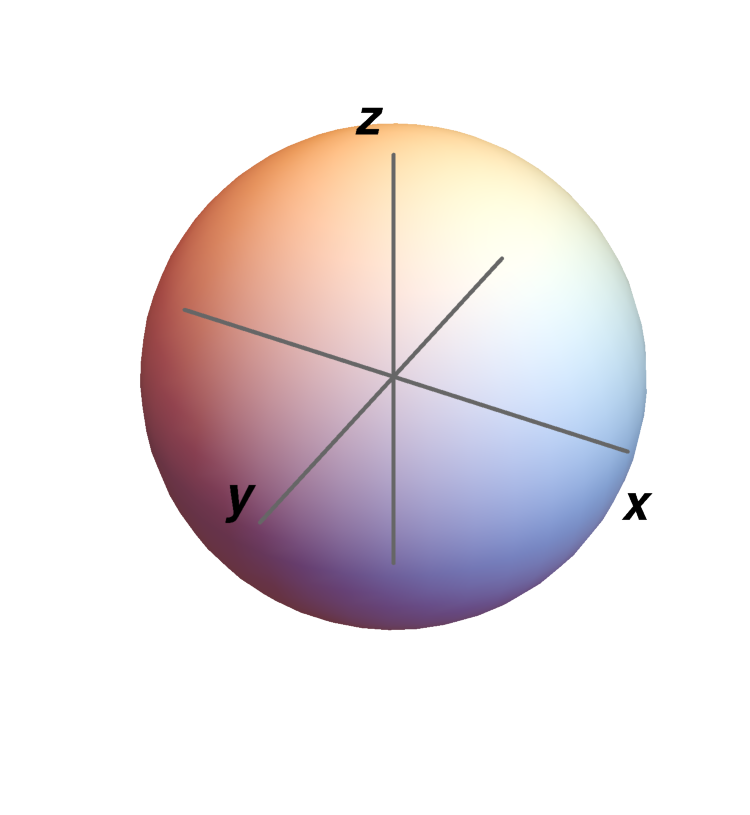
\includegraphics[width=6cm]{images/bloch-ball}
    \end{minipage}
    $\longmapsto$
    \begin{minipage}{0.4\textwidth}
        \centering
        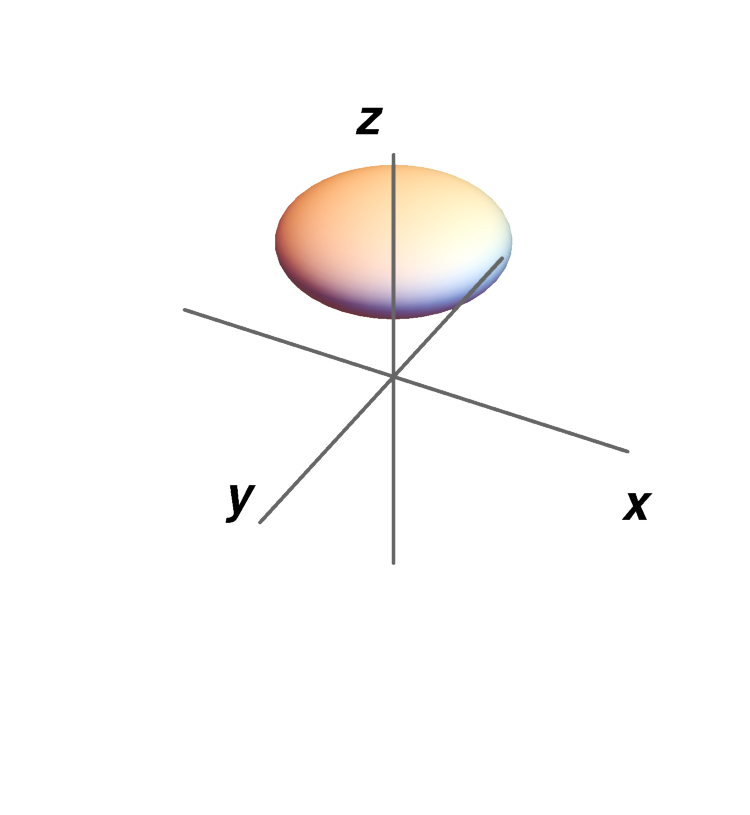
\includegraphics[width=6.2cm]{images/gen-amplitude-damping}
    \end{minipage}
    \caption{Efecto del canal generalizado de amortiguamiento de 
        amplitud sobre la esfera de Bloch, 
        para $p=0.4$.}
    \label{fig:amp-damp}
\end{figure}
Igual que en los ejemplos anteriores, la matriz de densidad $\rho'$
se infiere de \eqref{eq:damp-phase} y se calcula la representación 
matricial de $\E_{AF}$ en su forma de superoperador. De esa 
manera, se obtiene que la ecuación de transformación de la 
matriz de densidad es
\begin{align}
\mqty(
1 & 0 & 0 & \gamma  \\
0 & \sqrt{1-\gamma } & 0 & 0 \\
0 & 0 & \sqrt{1-\gamma } & 0 \\
0 & 0 & 0 & 1-\gamma
)
\frac{1}{2}
\mqty(
1+r_z\\r_x-ir_y\\r_x+ir_y\\1-r_z
)
=
\frac{1}{2}
\mqty(
1+\gamma+\qty(1-\gamma)z\\
\sqrt{1-\gamma}\qty(x-i y)\\
\sqrt{1-p}\qty(x+i y)\\
1-\gamma-\qty(1-\gamma)z
).
\end{align}
Se calcula la matriz de Choi de $\E_{AF}$ con la transformación
de \textit{reshuffle} y se obtienen sus autovectores multipicados
por la raíz cuadrada de sus autovalores asociados, reordenados
como matrices. Así, se obtiene que los operadores de Kraus 
del canal de amortiguamiento de amplitud son
\begin{align}
E_0&=
\sqrt{1-\gamma }
\mqty(
\frac{1}{\sqrt{1-\gamma }} & 0 \\
0 & 1
),&
E_1&=
\sqrt{\gamma }
\mqty(
0 & 1 \\
0 & 0 
).
\end{align}

Hemos expuesto 3 ejemplos de canales cuánticos de 1 qubit:
el canal de inversión de fase y bit, el canal depolarizante 
y el canal de amortiguamiento
de amplitud. La acción de los canales cuánticos de 1 qubit 
es más sencilla de visualizar en la representación de la esfera de Bloch
y su deformación bajo la acción del canal. 
El canal de inversión de fase y bit deforma la
esfera de Bloch de tal manera que encoge las componentes $x$ y $z$ en 
un factor $1-2p$ y deja invariante la componente
$y$ de cada punto en la esfera, con $p$ un parámetro que indica la
probabilidad de ocurrir una inversión de bit y fase de un estado. 
El canal depolarizante 
deforma todas las componentes del vector de Bloch de manera uniforme
en un factor $1-p$, es decir que la esfera de Bloch se encoge
continuamente hasta un punto en el origen, el estado
de máximamente mixto de un sistema de 1 qubit. Por último, 
el canal de amortiguamiento de amplitud deforma la esfera de Bloch
a un elipsoide cuyo centro geométrico no coincide con el origen. Por
ello, se dice que el canal no es unital. Los canales unitales son 
aquellos que dejan invariante el estado máximamente mixto, 
que en la representación de la esfera de Bloch se traduce en 
que la acción del canal no modifica el origen de coordenadas.

El formalismo de los canales cuánticos proporciona un marco 
teórico para describir el cambio dinámico de los estados cuánticos 
de sistemas que interactúan con su entorno. Una manera 
más intuitiva de llamar a los canales cuánticos es mapeos 
completamente positivos que preservan la traza, para enfatizar 
que los canales cuánticos son mapeos afines de matrices de 
densidad que transforman estados positivos en estados positivos,
sin importar la naturaleza del entorno con el que el sistema podría
interactuar. Dos formas de representar a los canales cuánticos
se presentaron en este capítulo, la forma de superoperador y 
la forma de Kraus, cuya conexión entre ambas representaciones
es posible mediante la matriz de Choi del canal cuántico. 
La preferencia por alguna representación u otra está determinada 
por la naturaleza del problema a resolver. 
En el siguiente capítulo veremos las ventajas de la forma de superoperador 
de un canal cuántico en el problema de estudio de este proyecto. 
% }}}
% }}}

